\section{QueryConditionedF and Heuristic Pre-Training}
\label{sec:query-conditioned-f}

\subsection{Free-energy functional}

For state \(\rho\) and query embedding \(q \in \mathbb{R}^{384}\):

\begin{equation}
F(\rho, q) = \underbrace{\sum_{s} D_{\mathrm{KL}}(\rho_s \,\|\, \pi_{\mathrm{prior},s})}_{\mathrm{complexity}}
         + \underbrace{\tfrac{1}{2\sigma^2} \| q - g_{\mathrm{JEPA}}(\rho) \|^2}_{\mathrm{accuracy\;(JEPA)}}
         + \underbrace{\lambda_J \sum_{s,t} J_{st} \langle \rho_s, \rho_t \rangle}_{\mathrm{coupling}}
\label{eq:F}
\end{equation}

The decoder \( g_{\mathrm{JEPA}} : \Delta^{128} \to \mathbb{R}^{384} \) is a two-layer MLP (128 \(\to\) 256 \(\to\) 384, GELU activations) with parameters pre-trained as described below. The prior \(\pi_{\mathrm{prior}, s}\) defaults to the uniform simplex; in our experiments we keep \(\sigma^2 = 1\) and \(\lambda_J = 0.1\). The species coupling matrix \(J \in \mathbb{R}^{4 \times 4}\) is taken from the Levelt-Baddeley specification used by \texttt{T2FreeEnergy} in our codebase.

\subsection{Gradients}

The complexity term yields \( \partial_{\rho_s} = \log(\rho_s / \pi_{\mathrm{prior},s}) + 1 \) and the coupling term yields \( \partial_{\rho_s} = 2 \lambda_J \sum_{t} J_{s,t} \rho_t \), both analytical. The JEPA term is differentiated via JAX autodiff.

One JKO step minimizes \( F(\rho, q) + \tfrac{1}{2h} W_2^2(\rho, \rho_\tau) \), the Wasserstein formulation of variational inference. As \(\tau \to \tau+1\) the flow approximates the active-inference posterior \( q^\star(s \mid q) \).

\subsection{Heuristic labeler (phase A)}
\label{sec:labeler}

To pre-train \( g_{\mathrm{JEPA}} \) without ground-truth species labels, we build a deterministic French NLP labeler that maps each query \( q \) to a target \(\pi^{\mathrm{lbl}} \in (\Delta^{32})^4\):

\begin{itemize}
    \item \textbf{phono}: 32 phonetic classes (4 broad groups \(\times\) 8 finer subclasses) extracted via the espeak-ng backend of \texttt{phonemizer}.
    \item \textbf{sem}: 32 categorical semantic bins, currently keyed via a stable lemma hash (a placeholder for a WordNet-fr or KMeans-MiniLM mapping; this affects only the absolute identity of bins, not the simplex structure).
    \item \textbf{lex}: 32 log-frequency bins computed from Lexique.org 3.83~\cite{newboucard2004lexique}.
    \item \textbf{syntax}: 32 Universal Dependency labels, counted from a SpaCy-fr dependency parse.
\end{itemize}

Phase A then minimizes \( \| f_\theta(q) - g_{\mathrm{JEPA}}(\mathrm{flatten}(\pi^{\mathrm{lbl}})) \|^2 \) via Adam-W on \(\sim\)5--10k French queries; \( f_\theta \) is held fixed during phase A and selected by the encoder ablation reported in Section~\ref{sec:experiments}.

\subsection{Ablation}
\label{sec:ablation}

Figure~\ref{fig:ablation} reports the per-species KL on the FR hybrid
corpus at 10k (pilot) and 50k (scale) for three text encoders
(\(\mathrm{B}_{\text{distilled}}\), \(\mathrm{C}_{\text{hash-mlp}}\),
\(\mathrm{D}_{\text{tiny-tf}}\)). Figure~\ref{fig:scaling} plots the total
test KL trajectory \(10\text{k} \to 50\text{k}\) per architecture.
\(\mathrm{C}_{\text{hash-mlp}}\) retains rank-1 at both scales and the
gap to rank-2 \(\mathrm{B}_{\text{distilled}}\) collapses from
\(\approx 3\%\) at 10k to \(\approx 0.3\%\) at 50k, confirming the
R3 kill-switch promotion to Top-2.

\begin{figure}[t]
  \centering
  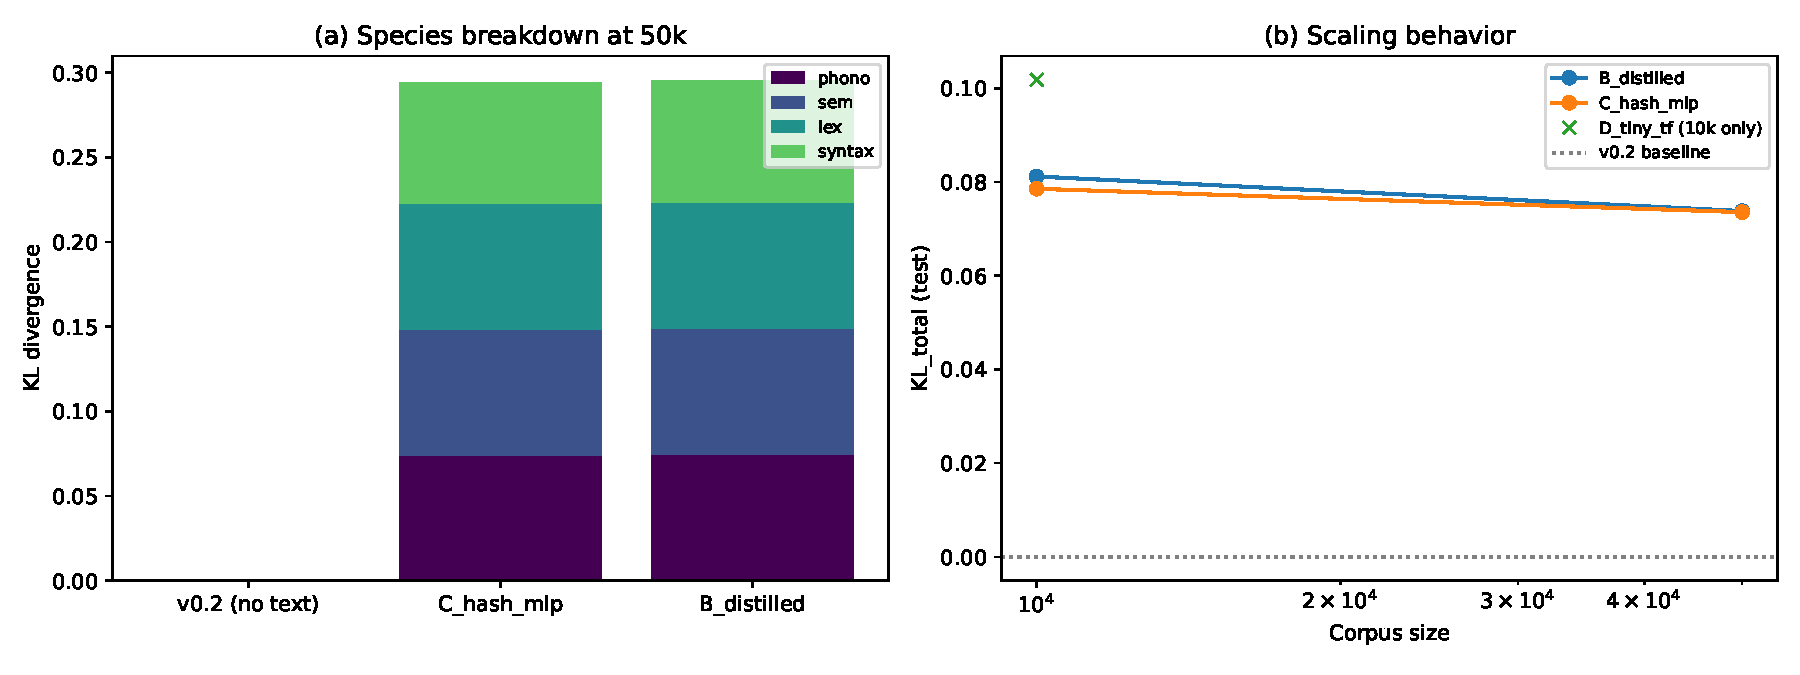
\includegraphics[width=\linewidth]{figures/ablation_kl_species.pdf}
  \caption{Per-species KL across encoders on pilot10k and scale50k.}
  \label{fig:ablation}
\end{figure}

\begin{figure}[t]
  \centering
  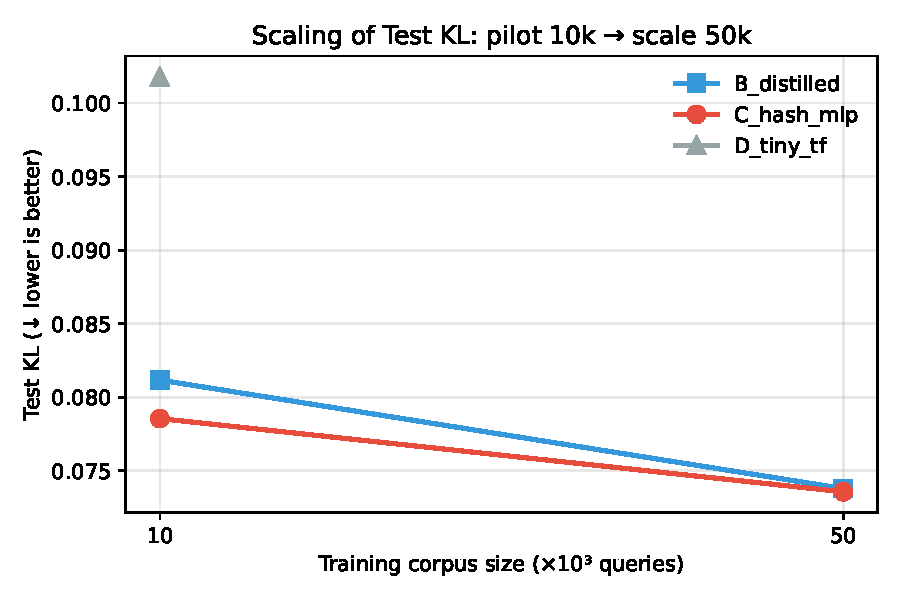
\includegraphics[width=0.75\linewidth]{figures/scaling_curves.pdf}
  \caption{Total test KL scaling \(10\text{k} \to 50\text{k}\) per
    architecture.}
  \label{fig:scaling}
\end{figure}
